% ભાગ: ગણો-વિધેયો-સંબંધો
% પ્રકરણ: અંકગણિતીકરણ
% વિભાગ: વાસ્તવિક સંખ્યાઓ

\documentclass[../../../include/open-logic-section]{subfiles}

\begin{document}

\olfileid{sfr}{arith}{real}
\olsection{વાસ્તવિક રેખા}

આગળનું પગલું સંમેય સંખ્યાઓમાંથી વાસ્તવિક સંખ્યાઓ કેવી રીતે રચવી તે
બતાવવાનું છે. એ પહેલાં વાસ્તવિક સંખ્યાઓની \emph{વિશિષ્ટતા} શી છે તે
સમજવું પડશે.

વાસ્તવિક સંખ્યાઓનો વ્યવહાર સંમેય સંખ્યાઓ જેવો જ છે. (પ્રાવિધિક રીતે,
બંને \emph{ક્રમિત ક્ષેત્રો}નાં ઉદાહરણો છે; તેની વ્યાખ્યા માટે
\olref[check]{orderedfield} જુઓ.) જો તમે \olref[sfr][siz][]{chap}ના
સ્વાધ્યાયો કર્યા હોય તો જાણતા હશો કે સંમેય સંખ્યાઓ કરતાં વાસ્તવિક
સંખ્યાઓ ચુસ્તપણે વધુ છે, એટલે કે $\cardless{\Rat}{\Real}$. કૅન્ટૉરે
સૌપ્રથમ આ સાબિત કર્યું હતું. પરંતુ લગભગ અઢી હજાર વર્ષથી જાણીતું છે કે
અસંમેય સંખ્યાઓ, એટલે કે સંમેય ન હોય એવી વાસ્તવિક સંખ્યાઓ, અસ્તિત્વ
ધરાવે છે. ખરેખર:
%\footnote{હવે: ``$\sqrt{2}$'' ધન અને ઋણ બંને વર્ગમૂળ દર્શાવે છે; પરંતુ આગળનાં થોડાં પાનાંમાં હું આ ભૂલીને માત્ર ધન વર્ગમૂળ વિચારીશ.}
\begin{thm}\ollabel{root2irrational}
$\sqrt{2}$ સંમેય નથી, એટલે કે $\sqrt{2} \notin \Rat$.
\end{thm}

\begin{proof}
વિરોધાભાસ માટે ધારો કે $\sqrt{2}$ સંમેય છે. તેથી કેટલીક પ્રાકૃતિક
સંખ્યાઓ $m$ અને $n$ માટે $\sqrt{2} = \nicefrac{m}{n}$. વળી $m$ અને
$n$ને એ રીતે પસંદ કરી શકાય કે અપૂર્ણાંકને વધુ સાદો ન કરી શકાય.
ફેરગોઠવણી કરતાં $m^{2} = 2n^{2}$. અહીંથી સાબિતી બે રીતે પૂરી કરી શકાય:

\emph{પહેલી, ભૌમિતિક રીતે} (ટેનેનબાઉમને અનુસરીને).\footnote{આ સાબિતી
\cite{Conway2006}માં નોંધાયેલી છે.} આ ચોરસો વિચારો:
\begin{center}
  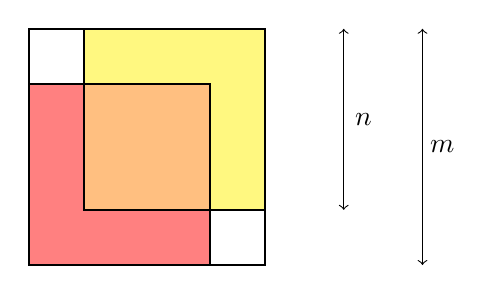
\begin{tikzpicture}
    \draw[thick] (0,0) rectangle (3,3);
    \draw[thick, fill=red!50] (0,0) rectangle (2.3,2.3);
    \draw[thick, fill=yellow!50] (0.7,0.7) rectangle (3, 3);
    \draw[thick, fill=orange!50] (0.7,0.7) rectangle (2.3, 2.3);
    \draw[<->] (4, 0.7)--(4, 3);
    \node at (4.25, 1.85) (n) {$n$};
    \draw[<->] (5, 0)--(5, 3);
    \node at (5.25, 1.5) (m) {$m$};
  \end{tikzpicture}
\end{center}
$m^2 = 2n^2$ હોવાથી $n$ બાજુવાળા બંને ચોરસો જ્યાં પરસ્પર આવરે છે
તે પ્રદેશનું ક્ષેત્રફળ બંને ચોરસોમાંથી કોઈ પણ ન આવરે એવા પ્રદેશના
ક્ષેત્રફળ જેટલું છે; એટલે કે નારંગી ચોરસનું ક્ષેત્રફળ છાયા વિનાના બે
ચોરસોનાં ક્ષેત્રફળોના સરવાળા જેટલું છે. તેથી નારંગી ચોરસની બાજુ $p$
અને છાયા વિનાના દરેક ચોરસની બાજુ $q$ હોય તો $p^2 = 2q^2$. પરંતુ હવે
$p < m$, $q < n$, $p, q \in \Nat$ સાથે
$\sqrt{2} = \nicefrac{p}{q}$. આ $m$ અને $n$ને શક્ય તેટલા નાના પસંદ
કર્યા હતા એ હકીકતનો વિરોધ કરે છે.

\emph{બીજી, ઔપચારિક રીતે.} $m^{2} = 2n^{2}$ હોવાથી $m$ યુગ્મ છે.
($x$ અયુગ્મ હોય તો $x^2$ અયુગ્મ છે તે બતાવવું સરળ છે.) તેથી કોઈ
$r \in \Nat$ માટે $m = 2r$. ફેરગોઠવણી કરતાં $2r^2 = n^2$,
    %                \begin{align*}
    %                  (2q)^{2} &= 2n^{2}\\
    %                  4q^{2} &= 2n^{2}\\
    %                  2q^{2} &= n^{2}
    %                \end{align*}
એટલે $n$ પણ યુગ્મ છે. આથી $m$ અને $n$ બંને યુગ્મ છે અને તેથી
$\nicefrac{m}{n}$ અપૂર્ણાંકને \emph{વધુ} સાદો કરી શકાય છે.
વિરોધાભાસ!
\end{proof}

પ્રસંગોપાત, આ આકૃતિમય સાબિતી આપણને \olref[his][set][mythology]{sec}ની
સામગ્રી ફરી વિચારવા દે છે. ટેનેનબાઉમ (1927--2006) પૂરેપૂરા આધુનિક
ગણિતજ્ઞ હતા; છતાં આ સાબિતી નિર્વિવાદપણે સુંદર, સંપૂર્ણ ચુસ્ત અને
ભૌમિતિક અંતઃપ્રજ્ઞા પર આધારિત છે!

કોઈ પણ રીતે જુઓ તો વાસ્તવિક સંખ્યાઓ સંમેય સંખ્યાઓ કરતાં ``વધુ
વિસ્તૃત'' છે. એક અર્થમાં સંમેય સંખ્યાઓમાં ``ખાલી જગ્યાઓ'' છે અને
વાસ્તવિક સંખ્યાઓ તે ભરે છે. વાયર્સ્ટ્રાસે સમજ્યું કે આ વાત વાસ્તવિક
સંખ્યાઓનો એક જ એવો ગુણધર્મ વર્ણવે છે જે તેમને સંમેય સંખ્યાઓથી જુદી
પાડે છે—એટલે પૂર્ણતા ગુણધર્મ: \emph{ઉચ્ચસીમા ધરાવતા વાસ્તવિક
સંખ્યાઓના દરેક અખાલી ગણને ન્યૂનતમ ઉચ્ચસીમા હોય છે.}

સંમેય સંખ્યાઓ પૂર્ણતા ગુણધર્મ ધરાવતી નથી તે સહેલાઈથી જોઈ શકાય છે.
દાખલા તરીકે $\sqrt{2}$ કરતાં નાની સંમેય સંખ્યાઓનો ગણ વિચારો, એટલે કે:
\[
  \Setabs{p \in \Rat}{p^2 < 2 \text{ અથવા }p < 0}
\]
આ ગણને સંમેય સંખ્યાઓમાં ઉચ્ચસીમા છે; દાખલા તરીકે તેના !!{element}s<
બધા $3$ કરતાં નાના છે. પરંતુ તેની ન્યૂનતમ ઉચ્ચસીમા શી છે? આપણે
`$\sqrt{2}$' કહેવા ઇચ્છીએ; પરંતુ હમણાં જ જોયું કે $\sqrt{2}$
\emph{સંમેય નથી}. અને $\sqrt{2}$ કરતાં મોટી કોઈ \emph{ન્યૂનતમ}
સંમેય સંખ્યા નથી. તેથી આ ગણને ઉચ્ચસીમા છે પરંતુ ન્યૂનતમ ઉચ્ચસીમા નથી.
પરિણામે સંમેય સંખ્યાઓ પૂર્ણતા ગુણધર્મ ધરાવતી નથી.

તેનાથી વિપરીત, સાતત્યક ``તાત્ત્વિક રીતે'' પૂર્ણતા ગુણધર્મ ધરાવવું
જોઈએ. આપણે માત્ર $\sqrt{2}$ને વાસ્તવિક સંખ્યા બનાવવા નથી ઇચ્છતા;
સંમેય રેખાની બધી ``ખાલી જગ્યાઓ'' ભરવા ઇચ્છીએ છીએ. ખરેખર, સાતત્યકમાં
પોતે કોઈ ``ખાલી જગ્યા'' ન રહે એવું ઇચ્છીએ છીએ. પૂર્ણતા વડે આપણને
બરાબર આ જ મળશે.

\end{document}
